\addtocontents{toc}{\protect\newpage}

\chapter{Концептуальна модель \\ системи доведення теорем}
Другий розділ описує розвиток концептуальної моделі системи доведення теорем як сукупності:
i) середовища виконання, яке складається з інтерпретатора та операційної системи;
ii) послідовності формальних мов програмування,
кожна наступна з яких, складніша за попередню,
має свою операційну семантику, та наслідує усі властивості
попередніх мов послідовності.

\section{Попередні відомості та теорії}
Для розповіді про систему доведення теорем, як систему мов програмування
будемо використовувати теорію категорії та теорію індуктивних
типів для специфікації синтаксисів мов програмування. Перелік необхідних формальних теорій:
лямбда числення, теорії індуктивних типів, вищі рівності для гомотопічної системи
тощо, містяться в розділі 3. Формальна теорія категорії міститься у розділі 4.
Слід зауважити, що ця формалізація проводиться на основі гомотопічної
мови програмування побудованої в даному розділі 2.

\begin{definition} (Концепт, Готлоб Фреге).
Концепт --- це предикат над об'єктом,
або іншими словами залежний $\Pi$-тип з теорії типів Мартіна-Льофа.
Об'єкт $x : o$ належить до концепту, тільки якщо сам концепт,
параметризований цим об'єктом, населений $p(o) : U$, де $p : concept(o)$.
\end{definition}

\begin{definition} (Система).
Визначимо систему як сукупність об'єктів $Ob : U$
та зв'язків між ними $Hom : Ob \rightarrow Ob \rightarrow U$.
\end{definition}

\begin{definition} (Концептуальна модель).
Таким чином концептуальна модель визначається як категорія, об'єкти якої
індексовані певною множиною, або залежні від параметра.
\end{definition}

\begin{definition} (Синтаксичне дерево).
Синтаксичне дерево --- це індуктивний тип або дерево Бома,
контруктори якого відповідають одному з 5 правил в теорії типів,
як правило використовуються три правила: правило формації, інтро-правила та елімінатор.
\end{definition}

\begin{definition} (Вище синтаксичне дерево).
Синтаксичне дерево в яке додано $\beta$ та $\eta$ правила називається
вищим синтаксичним деревом.
\end{definition}

\begin{definition} (Мова програмування).
Мова програмування або мовна категорія --- це категорія,
об’єкти якої --- це maybe-типи сум синтаксичних дерев мов програмування,
  а морфізми --- це стрілки (які містять правила виводу, типизації, нормалізації, екстакції тощо).
Приклади синтаксичних дерев: $O_\Pi$, $O_\Sigma$, $O_=$.
Приклади мовних категорій: $O_{PTS}$, $O_{MLTT}$, $O_{HTS}$.
\end{definition}

\begin{definition} (Модель).
Модель визначимо як систему формальних мов (об'єкти) разом з їх програмами,
та мовними перетвореннями (звязки) між ними для яких працює правило асоціативності
композиції та правила лівої і правої композиції з одиничними стрілками.
Іншими словами будемо розуміти тут категорну модель.
\end{definition}

\begin{definition} (Послідовність синтаксичних дерев). Кожна послідовність
синтаксичних дерев
\begin{equation}
O_\Pi \rightarrow O_\Sigma \rightarrow O_= \rightarrow O_W \rightarrow O_I.
\end{equation}
генерує відповідну послідовність мов програмування
\begin{equation}
\begin{split}
O_{PTS}(O_\Pi) \rightarrow O_{CTX}(O_\Pi,O_\Sigma) \rightarrow O_{EQU}(..,O_\Sigma,O_=) \rightarrow \\
 \quad \rightarrow O_{ITS}(...,O_=,O_W) \rightarrow O_{HTS}(...,O_W,O_I).
\end{split}
\end{equation}
наступним чином. Кожна мова програмування залежить
від синтаксису який її визначає
та всіх попредніх синтаксисів мов програмування з послідовності.
Перша мова програмування містить тільки перший синтаксис.
Розкриті сигнатури мають вигляд:
$O_{PTS}: O_\Pi \rightarrow U$,
$O_{CTX}: O_\Pi \rightarrow O_\Sigma \rightarrow U$,
$O_{EQU}: O_\Pi \rightarrow O_\Sigma \rightarrow O_= \rightarrow U$,
$O_{ITS}: O_\Pi \rightarrow O_\Sigma \rightarrow O_= \rightarrow O_W \rightarrow U$,
$O_{HTS}: O_\Pi \rightarrow O_\Sigma \rightarrow O_= \rightarrow O_W \rightarrow O_I \rightarrow U$.
\end{definition}

Таким чином кожна наступна мова програмування містить усі попередні
мови програмування, визначені послідовністю синтаксичних дерев,

\begin{definition} (Створення мовної категорії).
Мови можна додавати, наприклад $O_{HTS} = O_{\Pi\Sigma=WI}$, для побудови якої необхідно
об'єднати у індуктивному типі мови усі індуктивні типи її підмов.
Таким чином функтор діє на декартовому добутку синтаксичних дерев мовних категорій
та має значення в категорій мовних категорій. Приклад найпотужнішої гомотопічної мови:
\begin{equation}
O_{HTS} = O_{\Pi\Sigma=WI} : O_\Pi \rightarrow O_\Sigma \rightarrow O_= \rightarrow O_W \rightarrow O_I \rightarrow U.
\end{equation}
\end{definition}

Кожне синтаксичне дерево, як правило, містить конструктори
та елімінатори певного одного типу. Але починаючи з $O_{ITS}$
складність типів, які додаються до ядра значно зростає.
Таким чином мовні категорії конструються гранулярно з
точністю до включення певного типу в ядро верифікатора.

\begin{definition} (Типи синтаксичних дерев).
У розділі 1 були проаналізовані усі мови програмування та середовища виконання,
а також спеціалізовані мови моделювання. В результаті чого було встановлено
чітки індивідуальні мовні синтаксиси. Кожен синтаксис складається з
множини синтаксичних одиниць цієї мови (конструктори індуктивного типу),
які відповідають правилам теорії типів Мартіна-Льофа (формації, інтро-правило,
елімінатор, $\beta$-, та $\eta$-правила). Якщо додати $\beta$-, та $\eta$-правила
як рівності у визначення синтаксису, то для представлення потрібні вищі індуктивні типи.
Таким чином кожному синтаксичному дереву відповідає певний тип в теорії типів Мартіна-Льофа.
\begin{table}
\centering
  \caption{Кластерний аналіз мовних синтаксисів}
 \begin{tabular}{lcccc}
    \hline
       Синтаксис & Мова програмування або її підмова \\
    \hline
       $O_\lambda$ & Нетипизоване $\lambda$-числення Чорча \\
       $O_\pi$     & Числення процесів, CCS, CSP або $\pi$-числення Мілнера\\
       $O_\mu$     & Тензорне числення та векторизація \\
    \hline
       $O_\Pi$     & Числення конструкцій (функціональна повнота) \\
       $O_\Sigma$  & Числення контекстів (контекстуальна повнота) \\
       $O_=$       & Теорія типів Мартіна-Льофа (логіка) \\
       $O_W$       & Числення індуктивних конструкцій (матіндукція) \\
       $O_I$       & Гомотопічна система типів (формальна математика) \\
      \hline
  \end{tabular}
\end{table}
\end{definition}

\begin{definition} (Спектральна категорія мов).
Так, виділяється наступна послідовність мов, та функторів між ними,
де кожна мова-кодомен є складнішою та біль потужною за мову-домен.
Система мов є категорією мовних категорій або категорією мов програмування.
\begin{equation}
O_\infty : O_{CPS} \rightarrow O_{PTS} \rightarrow O_{MLTT} \rightarrow O_{ITS} \rightarrow O_{HTS} \rightarrow ...
\end{equation}
\end{definition}

\begin{definition} (Коконтекстуальна категорія мов).
Якщо не виділяти певну послідовність мовного ускладнення та розглядати
усі суми усієї певної множини мовних синтаксисів, то ми отриміємо коконтекстуальну категорію,
де об'єкти --- це усі можливі мовні категорії побудовані за допомогою усіх перестановок суми мовних синтаксисів,
а морфізми це функтори перетворення однієї мовної категорії в іншу мовну категорію.
Приклади: $O_{I*} \rightarrow O_{\Pi=}$, $O_\Pi \rightarrow O_{\Pi\Sigma}$,
$O_\Pi \rightarrow O_{\Pi\Sigma}$, $O_{\Pi*} \rightarrow O_\Pi$.
\end{definition}

\section{Структурне представлення моделі}
Виходячи з визначення моделі, вони можуть мати різний
набір об'єктів в системі мов програмування.
Покажемо приклади ексземплярів які можно породити в рамках цієї моделі.

\subsection{Мінімальна система}
Приклад мінімальної системи, яка містить лише одну мову для доведення теорем
та одну мову для виконання програм.

\begin{equation}
PTS_{CPS} = 
\begin{cases}
Ob: \{ O_{CPS}, O_{PTS} \} \\
Hom: \{ 1,2: \mathbb{1} \rightarrow O_{PTS}, 3: O_{PTS} \rightarrow O_{CPS} \}
\end{cases}
\end{equation}

Стрілки 1 та 2 визначають
модель та базову бібліотеку, а стрілка 3 означає екстракт
доведення (якщо таке є) в інтерпретатор. Можна використати графічну
мову мереж Петрі для зображення екземпляра моделі системи мов.

\begin{figure}
  \centerline{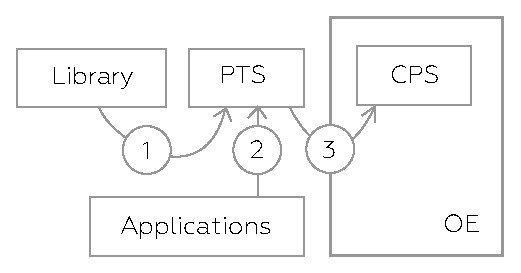
\includegraphics[scale=0.6]{minimal.eps}}
  \caption{Мінімальна система з чистої мови та інтерпретатора}
\end{figure}

\subsection{Максимальна система}
Інший приклад системи --- це максимальна система, яка містить усі формальні
мови програмування та формальне середовище виконання (порядок синтаксичних дерев
як параметрів при конструюванні мовної категорії може змінюватися, тут
генеалогія HTS не ведеться від MLTT, яке є розгалуженням).
\begin{equation}
Total = 
\begin{cases}
Ob: \{ O_{CPS}, O_{PTS}, O_{MLTT}, O_{ITS}, O_{HTS} \} \\
Hom: \begin{cases}
1,2: \mathbb{1} \rightarrow O_{HTS}, 3: O_{MLTT} \rightarrow O_{ITS} \\
4: O_{HTS} \rightarrow O_{ITS}, 5: O_{ITS} \rightarrow O_{PTS}, 6: O_{PTS} \rightarrow O_{CPS}
\end{cases}
\end{cases}
\end{equation}
За допомогою мереж Петрі це можна відобразити наступним чином:
\begin{figure}[ht]
  \centerline{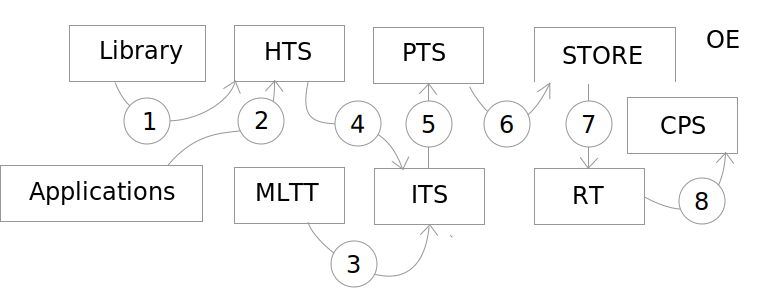
\includegraphics[scale=0.6]{full.eps}}
  \caption{Кубічна та чиста системи типів та середовище виконання}
\end{figure}

\section{Формальні мови програмування}
Тут йдеться про мови програмування придатні для доведення теорем,
та їх таксономію від найелементарніших (чистої системи з одним типом $\Pi$) до
найпотужніших гомотопічних систем. Одна така гомотопічна система є кінцевим завданням
цього розділу --- побудова моделі гомотопічного верифікатора.
В процесі його побудови в цьому розділі ми розглянемо під
мікроскопом складові частини його нижчих мовних рівнів.

Застосуємо категорну семантику для мов програмування і будемо розглядати
мови програмування як моноїдальні мовні категорі, об'єкти яких є просторами
усіх програм цих мов програмування, а морфізми --- правила верифікації та компіляції цих мов.
Морфізми між мовними категоріями в категорї мов програмування --- це
функтори підвищення та пониження складності мови, подібно до того як діють
морфізми в контекстуальних категоріях. Морфізм деконструює або конструює за
допомогою Either-типу або $\Sigma$-типу індуктивний тип мови програмування.

Мови розкладаються у спектральну (індексовану натуральними числами $N \rightarrow U$)
послідовність мов, кожен елемент якої є мовою програмування,
яка не містить синтаксичне дерево вищої мови програмування.

\subsection{Чиста система типів $O_{PTS}$}

Чиста ситема або числення конструкцій або система з одим типом або
система з однією аксіомою, продовжує традиції елементарних пруверів
в стилі першого AUTOMATH та сучасних Henk, Morte, Cedile, Om.

\begin{definition} (Мовна категорія чистої мови $O_{PTS}$).
\begin{equation}
O_{PTS} =
\begin{cases}
Ob: \{\ X: maybe\ PTS, target: maybe\ CPS \ \} \\
Hom: \begin{cases}
type,norm: X \rightarrow X, extract: X \rightarrow target \\
certify: X \rightarrow target = type \circ norm \circ extract
\end{cases}
\end{cases}
\end{equation}
\end{definition}

\begin{definition} (Синтаксис мовної категорії $O_{PTS}$).
Чиста мова $O_{PTS}$ містить лише синтаксис одного типу, $\Pi$-типу.
Така теорія називається теорією з одним типом, або з однією аксіомою.
\begin{lstlisting}
data PTS = ppure (_: pts PTS)
\end{lstlisting}
\end{definition}

Вона описана в літературі як Calculus of Construction (Кокан),
Pure Type System (Стемп, Фу).

\begin{definition} (Синтаксичне дерево $O_\Pi$).
\begin{lstlisting}[mathescape=true]
data pts (lang: U)
   = star (n: nat)
   | var (x: name) (l: nat)
   | pi (x: name) (l: nat) (f: lang)
   | lambda  (x: name) (l: nat) (f: lang)
   | app (f a: lang)
\end{lstlisting}
\end{definition}

\subsection{Теорія типів Мартіна-Льофа $O_{MLTT}$}

Мова теорії типів є сучасною основою всіх пруверів з залежними типами,
такими, наприклад, як NuPRL та Agda. Багато так званих $\Pi\Sigma$ пруверів
імплементують $MLTT$ серед таких як:
$\Pi\Sigma$\footnote{\url{https://github.com/zlizta/pisigma-0-2-2}},
$\Pi\forall$\footnote{\url{https://github.com/sweirich/pi-forall}}.

\begin{definition} (Мовна категорія $O_{MLTT}$).
\begin{equation}
O_{MLTT} =
\begin{cases}
Ob: \{\ maybe\ MLTT\ \} \\
Hom: \begin{cases}
type,norm: Ob \rightarrow Ob \\
certify: Ob \rightarrow Ob = type \circ norm
\end{cases}
\end{cases}
\end{equation}
\end{definition}

\begin{definition} (Синтаксис мовної категорії $O_{MLTT}$).
Мова $O_{MLTT}$ включає в себе синтаксиси трьох типів
теорії Мартіна-Льофа: $O_\Pi$, $O_\Sigma$, $O_=$.
\begin{lstlisting}
data MLTT = mpure (_: pts MLTT)
          | msigma (_: exists MLTT)
          | mid (_: identity MLTT)
\end{lstlisting}
\end{definition}

\begin{definition} (Синтаксичне дерево $O_\Sigma$).
Також можна до чистої системи додати $\Sigma$-тип,
піднявши типову систему до мови $O_{MLTT-72}$ або $O_{\Pi\Sigma}$ :
\begin{lstlisting}[mathescape=true]
data exists (lang: U)
   = sigma (n: name) (a b: lang)
   | pair (a b: lang)
   | fst (p: lang)
   | snd (p: lang)
\end{lstlisting}
\end{definition}

\begin{definition} (Синтаксичне дерево $O_=$).
Додавши тип рівності можно підняти систему ще на одну сходинку,
до $O_{MLTT-84}$ або $O_{\Pi\Sigma=}$:
\begin{lstlisting}[mathescape=true]
data identity (lang: U)
   = id (t a b: lang)
   | id_intro (a b: lang)
   | id_elim (a b c d e: lang)
\end{lstlisting}
\end{definition}

\subsection{Система індуктивних типів $O_{ITS}$}

\begin{definition} (Мовна категорія $O_{ITS}$).
\begin{equation}
O_{ITS} =
\begin{cases}
Ob: \{\ X: maybe\ ITS, target: maybe\ CPS\ \} \\
Hom: \begin{cases}
type,norm,induction: X \rightarrow X, extract: X \rightarrow target \\
certify : X \rightarrow target \\
cerfity = type \circ norm \circ induction \circ extract \\
\end{cases}
\end{cases}
\end{equation}
\end{definition}

Мова індуктивних типів дозволяє безпосередньо кодувати індуктивні типи,
не використовуючи схеми кодування Бома, містить усі попередні мовні синтаксиси:
$O_=$, $O_\Sigma$, $O_\Pi$.

\begin{definition} (Синтаксичне дерево мовної категорії $O_{ITS}$).
\begin{lstlisting}
data ITS = ipure (_: pts ITS)
         | isigma (_: exists ITS)
         | iid (_: identity ITS)
         | iITS (_: ind ITS)
\end{lstlisting}
\end{definition}

Мова містить наступні допоміжні визначення: i) телескопу,
який містить послідовність елементів мови; ii) розгалуження,
як конструкцій case оператора; iii) імен конструкторів індуктивного типу.

\begin{lstlisting}
data tele   (A: U) = emp | tel (n: name) (b: A) (t: tele A)
data branch (A: U) =        br (n: name) (args: list name) (term: A)
data label  (A: U) =       lab (n: name) (t: tele A)
                         | com (n: name) (t: tele A) (dim: list name)
                               (s: list  (prod (prod name bool) A))
\end{lstlisting}

\begin{definition} (Синтаксичне дерево $O_*$).
Правило формації, конструктора та елімінатора визначається синтаксичним деревом $O_*$:
\begin{lstlisting}
data ind (lang: U)
   = datum  (n: name) (t: tele lang) (labels:   list (label lang))
   | case   (n: name) (t: lang)      (branches: list (branch lang))
   | ctor   (n: name)                (args:     list lang)
\end{lstlisting}
\end{definition}

\subsection{Гомотопічна система типів $O_{HTS}$}

\begin{definition} (Мовна категорія $O_{HTS}$).
$$
O_{HTS} =
\begin{cases}
Ob: \{\ maybe\ HTS\ \} \\
Hom: \begin{cases}
type,norm: Ob \rightarrow Ob \\
certify: Ob \rightarrow Ob = type \circ norm \\
\end{cases}
\end{cases}
$$
\end{definition}

\begin{definition} (Синтаксис мовної категорії $O_{HTS}$).
Синтаксис гомотопічної мовної категорії містить усі
попередні мовні синтаксиси: $O_I$, $O_W$, $O_=$, $O_\Sigma$, $O_\Pi$:
\begin{lstlisting}
data HTS = hpure (_: pts HTS)
         | hsigma (_: exists HTS)
         | hid (_: identity HTS)
         | hind (_: ind HTS)
         | homotopy (_: hts HTS)
\end{lstlisting}
\end{definition}

Гомотопічна типа наслідує $O_{ITS}$ але модифіковану з
Path-типом в індуктивних визначеннях, структурою композиції,
анонсує Path-тип (формація, конструктор, та елімінатор)
як лямбда функцію на відрізку, а також склейку типів у всесвіті
та склейку змінних з відповідними елімінаторами.

\begin{definition} (Синтаксичне дерево $O_I$).
\begin{lstlisting}
data hts (lang: U)
   = path (t a b: lang)
   | plam (n: name) (a: alg) (b: lang)
   | papp (f: name) (a: lang) (p: alg)
   | comp_ (a b: lang)
   | fill_ (a b c: lang)
   | glue_ (a b c: lang)
   | glue_elem (a b: lang)
   | unglue_elem (a b: lang)
\end{lstlisting}
\end{definition}

Таким чином,
$O_{HTS}$ містить два Id-типа, один унаслідований від $O_=$,
а інший який міститься в синтаксичному дереві $O_I$.

\section{Формальне cередовище виконання}
Формальне середовище виконання складається з інтерпретатора
(нетитизованого $\lambda$-числення) та числення акторів (процесів, черг, таймерів).
Інтерпретатор та операційна система включені в систему доведення теорем
для уніфікації всіх сигнатур системи та формалізації самого інтерпретатора
як системи виконання. Слід зазначити, що не
завжди є змога зробити екстракт в $O_{CPS}$, тому об'єкти мовних
категорій є $maybe$-типами.
$$
O_{CPS}: O_\lambda \rightarrow O_\pi \rightarrow O_\mu \rightarrow U
$$
Далі буде йтися тільки про формальні інтерпретатори,
так як вони є найбільш компакними формами мов для
верифікації (в порівнянні з моделями System F).
Таким чином будемо розглядати формальне середовище виконання, як
сукупність інтерпретатора та операційної системи.

В цьому розділі ми побудуємо надшвидку імплементацію інтерпретатора,
яка цілком, разом зі своїми програмами, розміщується в кеш-памяті
першого рівня процесора, та здатна до AVX векторизацій засобами мови Rust.
Як промислова опція, підтримується також екстракт
в байт-код інтерпретатора BEAM віртуальної машини Erlang.

\subsection{Категорія середовища виконання $O_{CPS}$}

\begin{definition} (Категорія середовища виконнання$O_{СPS}$).
$$
O_{CPS} =
\begin{cases}
Ob: \{\ maybe\ CPS\ \} \\
Hom: \{\ eval: Ob \rightarrow Ob\ \}
\end{cases}
$$
\end{definition}

Синтаксис середовища виконання може містити наступні синтаксиси:
$O_\lambda$, $O_\pi$, $O_\mu$.

\begin{definition} (Синтаксис мовної категорії $O_{HTS}$).
\begin{lstlisting}
data CPS = church (_: lambda CPS)
         | milner (_: pi     CPS)
         | tensor (_: mu     CPS)
\end{lstlisting}
\end{definition}

\begin{definition} (Синтаксичне дерево $O_\lambda$). Інтерпретатор визначається
своїм трьома конструкторами: номер змінної (індекс де Брейна),
лямбда функція та її апплікація:
\begin{lstlisting}
data lambda = var (x: nat)
            | lam (l: nat) (d: cps)
            | app (f a: cps)
\end{lstlisting}
Мовою інтерпретаторів є нетипизоване лямбда числення, однак в залежності
від складності інтерпретатора це дерево може виглядати по-різному.
\end{definition}

\begin{definition} (Синтаксичне дерево $O_\pi$).
Правило формації, конструктора та елімінатора визначається синтаксичним деревом $O_*$:
\begin{lstlisting}
data pi (lang: U)
   = process (protocol: lang)
   | spawn (cursors: lang) (core: nat) (program: lang)
   | snd (cursor: lang) (data: lang)
   | rcv (cursor: lang)
   | pub (size: nat)
   | sub (cursor: lang)
\end{lstlisting}
\end{definition}

Кожна секція цієї глави буде присвячена цим мовним компонентам
системи доведення теорем. В кінці розділу дається повна система, яка включає в себе усі
мови та усі мовні перетворення.

\section{Чиста система типів PTS$^\infty$}

IEEE\footnote{IEEE Std 1012-2016  --- V\&V Software verification and validation} стандарт
та регуляторні документи ESA\footnote{ESA PSS-05-10 1-1 1995 -- Guide to software verification and validation}
визначають інтрументи та підходи до виробничого процесу верифікації та валідації.
Найбільш розвинені та потужні засоби вимагають застосування математичних мов та нотацій.
Ера верифікованої математики була започаткована верифікатором AUTOMATH\cite{deBruijn83} (де Брейн) розробленого
під керівництвом де Брейна, а також розвиток теорії типів Мартіна-Льофа\cite{Lof84}.
Сьогодні ми маємо Lean, Coq, F*, Agda мови які використовують числення
конструкцій, Calculus of Constructions\cite{Coq88} (CoC)
та числення індуктивних типів (Calculus of Inductive Constructions\cite{Pfenning89} (CiC).
Пізніше учень де Брейна, Хенк Барендрехт класифікував послаблені чисті
системи типів по трьом осям та візуазізував це за допомогою лямбда-куба\cite{Henk93}.
Чисті мови програмування вже були імплементовані раніше
(Morte\footnote{Gabriel Gonzalez. Haskell Morte Library \url{https://github.com/Gabriel439/Haskell-Morte-Library}} Габріеля Гонзалеза, Henk\cite{Erik97} Еріка Мейера).
Чисті системи типів це системи з однм $\Pi$-типом (або ще і $\Sigma$ як в ECC\cite{Ore92}, Оре),
з можливими розширеннями, такими як PTS$^\infty$ з бескінечною кількістю всесвітів\cite{Tonpa18} (Сохацький),
Cedile з self-типами\cite{Fu14}\cite{Stump17} (Стамп, Фу), система з К-правилами\cite{Barthe95} (Барте).

Головна мотивація чистих систем -- це простота аналізу ядра верифікатора,
можливість застосування сильної нормалізації та довірена зовнішня верифікація
та сертифікація завдяки простоті верифікатора (type checker), це означає, що
алгоритм верифікації повинен бути настільки простим, аби можна було
просто імплементувати його на будь-якій мові програмування. Приклади застовування
тут можуть бути:
1) формальна мова блокчейн контрактів (Pluto
   \footnote{Rebecca Valentine. Formal Specification of the Plutus Core Language. 2017.
             \url{https://iohk.io/research/papers/#JT5XKNBP}});
2) сертифіковані обчислення для інтерпретаторів;
3) платіжні системи.

\subsection{Генерація сертифікованих програм}
Згідно ізоморфізму Каррі-Говарда-Ламбека або інтерпретації Брауера-Гейтінга-Колмогорова
існує взаємноознозначна відповідність між доведеннями теорем (або пруфтермами)
та лямбда функціями в теорії типів Мартіна-Льофа\cite{Lof84}.
Так як специфікація та доведення її відоповідності для певної програми
відбувається за допомогою мови з залежними типами, ми можемо екстрагувати
цільову імплементацію (зі стертою інформацією про типи) сертифікованої программи
в довільну мову програмування. У якості такої цільової мови підходять
майже усі інтерпретатор безтипового лямбда числення, такі як JavaScript,
Erlang, PyPy, LuaJIT, K.

Більш розвинені практики та підходи до кодогенерації та екстрагуванню
сертифікованих програм полягає у генерації С++ чи Rust програм, або програм
для нижчих систем лямюда-кубу, таких як System F або System F$_\omega$.
У цій роботі представлений екстракт в мову Erlang у якості цільового інтерпретатору.

\begin{table}[h]
\begin{center}
\caption{List of languages, tried as verification targets}
\tabcolsep7pt\begin{tabular}{lcccc}
\hline
{\bf Target} & {\bf Class} & {\bf Intermediate} & {\bf Theory}\\
\hline
JVM        & interpreter/native   & Java       & F-sub\footnote{System F wit bounded quantification}\\
JVM        & interpreter/native   & Scala      & System F-omega\\
CLR        & interpreter/native   & F\#        & System F-omega\\
GHC        & compiler/native      & Haskell    & System D\\
GHC        & compiler/native      & Morte      & CoC\\
GHC,OCaml  & compiler/native      & Coq        & CiC\\
O,BEAM     & interpreter          & Om         & PTS$^\infty$ \\
JavaScript & interpreter/native   & PureScript & System F\\
\hline
\end{tabular}
\end{center}
\end{table}

{\bf PTS синтаксиси}. Мінімальне ядро з однією аксіомою
сприймає декілька лямбда ситаксисів.
Перший синтаксис сумісний з системою програмування
$morte$\footnote{http://github.com/Gabriel439/Haskell-Morte-Library}, та походить від неї.
Інший синтаксис сумісний з синтаксисом $cubical$\footnote{http://github.com/mortberg/cubicaltt}.
Планувалося також підтримати синтаксис $caramel$\footnote{https://github.com/MaiaVictor/caramel}.

\begin{equation}
\begin{cases}
Sorts = U.\{i\},\ i : Nat\\
Axioms = U.\{i\} : U.\{inc\ i\}\\
Rules = U.\{i\} \leadsto U.\{j\} : U.\{max\ i\ j\}\\
\end{cases}
\end{equation}

Мова програмування Ом -- це мова з залежними типами, яка є розширенням
числення конструкцій (Calculus of Constructions, CoC) Тері Кокана. Саме з числення
конструкцій починається сучасна обчислювальна математика. В додаток до CoC,
наша мова Ом має предикативну ієрархію індексованих всесвітів. В цій мові немає
аксіоми рекурсії для безпосереднього визначення рекурсивних типів. Однак в цій мові
вцілому, рекурсивні дерева та корекурсія може бути визначена, або як кажуть, закодована.
Така система аксіом називається системою з однією аксіомою (або чистою системою), тому що в ній
існує тільки Пі-тип, а для кожного типу в теорії типів Мартіна Льофа існує п'ять
конструкцій: формація, інтро, елімінатор, бета та ета правила.

Усі терми підчиняються системі аксіом {\bf Axioms} всередині
послідовності всесвітів {\bf Sorts} та складність залежного
терму відповідає максимальній складності домена та кодомена
(правила {\bf Rules}). Таким чином визначається простір всесвітів,
та його конфігурація може бути записана згідно нотації
Барендрехта для систем з чистими типами:

Проміжна мова чистої системи типів Ом базується на мові
Henk\cite{Erik97}, вперше описаній Еріком Мейером та Саймоном Пейтоном Джонсом в 1997 році.
Пізніше Габріель Гонзалез імплементував на мові Haskell
верифікатор з посиланням на Henk, та використував кодування Бома для нерекурсивного
кодування рекурсивних індуктивних типів. Ця мова базується лише на $\Pi$-типі,
$\lambda$-функції, її елімінатора аплікації, $\beta$-редукції та $\eta$-експансії.
Дизайн мови Ом нагадує дизайн мов Henk та Morte.
Ця мова призначена бути максимально простою (повна імплементація займає 300 рядків),
формально верифікованою, здатною продукувати сертифіковані програми та
розповсюджувати їх за межі комп'ютера по мережах та недовірених каналах зв'язку,
та компілювати (верифікувати та екстрагувати) на цільових платформах за допомогою
тієї ж мови Ом, можливо імплементовоної на іншій мові програмування та вбудованої
в основну систему.

\subsection{Синтаксис}

Синтаксис PTS сумісний з численням конструкцій (CoC) Тері Кокана,
та такими мовами як Morte та Henk.
Однак в системі PTS присутній індекс для всесвітів який
представлений натуральними числами. Тут наведений синтаксис у BNF нотації

\begin{lstlisting}[mathescape=true]
     I := #list #nat
     U := * + * . #nat
     O := U + I + ( O ) + O O + O $\rightarrow$ O
        + $\lambda$ ( I : O ) $\rightarrow$ O
        + $\forall$ ( I : O ) $\rightarrow$ O
\end{lstlisting}

Тут + --- сумма виразів, '.' --- конкатенація терміналів без пробілу,
:= --- оператор визначення BNF-правила, \#empty, \#nat, \#list --- вбудовані типи BNF-нотації
--- синтаксичні елементи BNF нотації,
а *,:, $\rightarrow$, (, ), $\lambda$, $\forall$ -- термінали або синтаксичні елементи мови програмування.
Еквівалентне визначення як ініціальний об'єкт категорій $O_{PTS}$ або $O_\Pi$
який може вмістити цей синтаксис містить всі правила виводу
внутрішньої мови категорії.

\begin{lstlisting}[mathescape=true]
data pts (lang: U)
   = star             (n: nat)
   | var    (x: name) (l: nat)
   | pi     (x: name) (l: nat) (d c: lang)
   | remote (n: name) (n: nat)
   | lambda (x: name) (l: nat) (d c: lang)
   | app                       (f a: lang)
\end{lstlisting}

\subsection{Всесвіти}
Мова PTS$^\infty$ -- це лямбда числення з залежними типами вищого порядку,
розширення числення конструкцій Кокана, або системи P$_\omega$ Барендрехта,
з предикативною (імпредикативною) ієрархією індексованих всесвітів.
Це розширення мотивоване консистентністю\cite{Lof75} в залежній теорії типів та
неможливістю кодування парадоксів Жирара-Хуркенса-Рассела\footnote{Так званий парадокс голяра який виникає в системах $U : U$}. Також для
забезпечення консистентності в мові PTS відсутня аксіома \lstinline{Fixpoint}, хоча
за допомогою рекурсивного трактування конструктора \lstinline{remote},
така можливість зберігається.

$$
    \mathrm{U_0} : \mathrm{U}_1 : \mathrm{U}_2 : \mathrm{U}_3 : ...
$$

Де $\mathrm{U_0}$ --- імпредикативний всесвіт,
   $\mathrm{U_1}$ --- перший предикативний всесвіт,
   $\mathrm{U_2}$ --- другий предикативний всесвіт,
   $\mathrm{U_3}$ --- третій предикативний всесвіт і т.д.

\begin{equation}
\tag{S}
\dfrac
{o : Nat}
{U_o}
\end{equation}

\subsubsection*{Предикативні всесвіти}
Всі терми підпорядковуються системі аксіом А для послідовності всесвітів S.
Складність R залежності термів дорівнює максимальнії складної термів з
яких складаєтсья формула (або вираз мови). Система всесвітів описується
згідно SAR-нотації Барендрехта. Зауважте, що предикативні всесвіти
несумісні в Бом кодуванням, але ви можете переключати предикативність.

\[
\tag{$A_1$}
\dfrac{i: Nat, j: Nat, i < j}{U_i : U_j}
\]

\[
\tag{$R_1$}
\dfrac{i : Nat, j : Nat}{U_i \rightarrow U_j : U_{max(i,j)} }
\]

\subsubsection*{Імпредикативні всесвіти}
Стягуваний імпредикативний простір внизу ієрархії є єдиним можливим розширенням
предикативної ієрархії для того аби вона залишалась консистентною. Однак
в чистій системі типів PTS підтримується ієрархія бескінечних імпредикативних всесвітів.

\begin{equation}
\tag{$A_2$}
\dfrac
{i: Nat}
{U_i : U_{i+1}}
\end{equation}

\begin{equation}
\tag{$R_2$}
\dfrac
{i : Nat,\ \ \ \ j : Nat}
{U_i \rightarrow U_{j} : U_{j}}
\end{equation}

\subsection{Контексти}

Контексти моделюються словником з іменами змінних в верифікаторі.
Він може бути типизований як \lstinline{list Sigma}.
Правило елімінації тут не дається, після використання функції верифікації,
словник вивільняється з пам'яті.

\begin{equation}
\tag{Ctx-formation}
\dfrac
{}
{\Gamma : Ctx}
\end{equation}

\begin{equation}
\tag{Ctx-intro$_1$}
\dfrac
{\Gamma : Ctx}
{\emptyset : \Gamma}
\end{equation}

\begin{equation}
\tag{Ctx-intro$_2$}
\dfrac
{A : U_i,\ \ \ \ x : A,\ \ \ \ \Gamma : Ctx}
{(x : A)\ \vdash\ \Gamma : Ctx}
\end{equation}

\subsection{Операційна семантика}

Операційна семантика --- це правила обчислення,
або $\beta$-,$\eta$-правила фьюжену інтро-правила та елімінаторів.
для визначення яких необхідно визначити:
1) інтро-правила, їх тип (правило формації), та класс (тип правила формації);
2) правило елімінації та залежної елімінації (індукції).
Таким чином будемо вважати, що операційна семантика системи типів $O_{PTS}$
буде складатися з 5 правил: формації, інтро-правило,
залежний елімінатор (індукція), $\beta$-редукція або правило обчислення,
$\eta$-експансія або правило унікальності.

\begin{equation}
\tag{$\Pi$-formation}
\dfrac
{A:U_i\ ,\ x:A \vdash B : U_j}
{\Pi\ (x:A) \rightarrow B : U_{p(i,j)}}
\end{equation}

\begin{equation}
\tag{$\lambda$-intro}
\dfrac
{x:A \vdash b : B}
{\lambda\ (x:A) \rightarrow b : \Pi\ (x: A) \rightarrow B }
\end{equation}

\begin{equation}
\tag{$App$-elimination}
\dfrac
{f: (\Pi\ (x:A) \rightarrow B)\ \ \ a: A}
{f\ a : B\ [a/x]}
\end{equation}

\begin{equation}
\tag{$\beta$-computation}
\dfrac
{x:A \vdash b: B\ \ \ a:A}
{(\lambda\ (x:A) \rightarrow b)\ a = b\ [a/x] : B\ [a/x]}
\end{equation}

\begin{equation}
\tag{subst}
\dfrac
{\pi_1 : A\ \ \ \ u:A \vdash \pi_2 : B}
{[\pi_1/u]\ \pi_2 : B}
\end{equation}

Перелік теорем (специфікації) для чистої системи типів можуть бути
прямо вбудовані в теорію типів, таким чином ми отримуємо логічний фреймворк
для перевірки імплементації залежної теорії.

\begin{lstlisting}[mathescape=true]
PTS (A: U): U
  = (Pi_Former: (A -> U) -> U)
  * (Pi_Intro: (B: A -> U) -> ((a: A) -> B a) -> (Pi A B))
  * (Pi_Elim: (B: A -> U) (a: A) -> (Pi A B) -> B a)
  * (Pi_Comp1: (B: A -> U) (a : A) (f: Pi A B) ->
    Equ (B a) (Pi_Elim B a (Pi_Intro B f)) (f a))
  * ((B: A -> U) (a: A) (f: Pi A B) ->
    Equ (Pi A B) f (\(x:A) -> f x))
\end{lstlisting}

Доведення цих теорем дано в модулі базової бібліотеки розділу 3.
Також можна повитися на інші доведення \cite{Henk93}.
Рівняння обсислювальної семантики (бета та ета правила) визначаються
за допомогою Path-типів, які визначаються $O_=$ або $O_I$ мовним синтаксисом.

Ці рівняння обчислювальної семантики представлені тут як Path-тип в вищій мові.
В чистій системі типів PTS з бескінечною кількістю всесвітів ми додається в AST
remote конструктор для завантаження файлів з локального довіреного сховища.
Рекурсія по цьому конструктору заборонена.

Індекси де брейна діють локально в межах одного імені.
При додаванні існуючого імені в контекст збільшується індекс цього імені.
Таким чином PTS верифікатор чистої системи типів відрізняється від
канонічного приклада алгоритма верифікації CoC\cite{Coq88}. Він включає
наступні функції мовної категорії: {\bf підстановка},
{\bf зсув імені}, {\bf нормалізація} термів, {\bf рівність}
за визначенням та {\bf верифікація}.

\subsection{Перевірка типів}

Для перевірки типів застосовується наступний алгоритм верифікації, який є основаю
усіх залежних систем. В чистих системах потрібно бути обережним з \lstinline{remote}
конструктором. Він використовуються для завантаження типів з локального довіреного сховища.
При дозволі рекурсії по \lstinline{remote} конструктору можливо реалізувати
self-типи\cite{Stump17}\cite{Fu14}.

\begin{lstlisting}[mathescape=true]
type (:star,N)     D $\rightarrow$ (:star,N+1)
     (:var,N,I)    D $\rightarrow$ :true = proplists:is_defined N B, om:keyget N D I
     (:remote,N)   D $\rightarrow$ om:cache (type N D)
     (:pi,N,0,I,O) D $\rightarrow$ (:star,h(star(type I D)),star(type O [(N,norm I)|D]))
     (:fn,N,0,I,O) D $\rightarrow$ let star (type I D), NI = norm I
                         in (:pi,N,0,NI,type(O,[(N,NI)|D]))
     (:app,F,A)    D $\rightarrow$ let T = type(F,D),
                            (:pi,N,0,I,O) = T, :true = eq I (type A D)
                         in norm (subst O N A)
\end{lstlisting}

\subsection{Індекси де Брейна}
Зсув переіменовує змінну N в контексті P, тобто додає одиницю для лічильника цієї змінної.

\begin{lstlisting}[mathescape=true]
  sh (:star,X)     N P $\rightarrow$ (:star,X)
     (:var,N,I)    N P $\rightarrow$ (:var,N,I+1) when I >= P
                       $\rightarrow$ (:var,N,I)
     (:remote,X)   N P $\rightarrow$ (:remote,X)
     (:pi,N,0,I,O) N P $\rightarrow$ (:pi,N,0,sh I N P,sh O N P+1)
     (:fn,N,0,I,O) N P $\rightarrow$ (:fn,N,0,sh I N P,sh O N P+1)
     (:app,L,R)    N P $\rightarrow$ (:app,L,R)
\end{lstlisting}

\subsection{Підстановка, нормалізація, рівність}
Підстановка заміняє змінну у виразі на певний терм.

\begin{lstlisting}[mathescape=true]
 sub (:star,X)     N V L $\rightarrow$ (:star,X)
     (:var,N,L)    N V L $\rightarrow$ V
     (:var,N,I)    N V L $\rightarrow$ (:var,N,I-1) when I > L
     (:remote,X)   N V L $\rightarrow$ (:remote,X)
     (:pi,N,0,I,O) N V L $\rightarrow$ (:pi,N,0,sub I N V L,sub O N (sh V N 0) L+1)
     (:pi,F,X,I,O) N V L $\rightarrow$ (:pi,F,X,sub I N V L,sub O N (sh V F 0) L)
     (:fn,N,0,I,O) N V L $\rightarrow$ (:fn,N,0,sub I N V L,sub O N (sh V N 0) L+1)
     (:fn,F,X,I,O) N V L $\rightarrow$ (:fn,F,X,sub I N V L,sub O N (sh V F 0) L)
     (:app,F,A)    N V L $\rightarrow$ (:app,   sub F N V L,sub A N V L)
\end{lstlisting}

Нормалізація виконує підстановку при аплікаціях до функцій (бета-редукція)
за допомогою рекурсивного спуску по конструкторам синтаксичного дерева.

\begin{lstlisting}[mathescape=true]
norm (:star,X)     $\rightarrow$ (:star,X)
     (:var,X)      $\rightarrow$ (:var,X)
     (:remote,N)   $\rightarrow$ cache (norm N [])
     (:pi,N,0,I,O) $\rightarrow$ (:pi,N,0,norm I,norm O)
     (:fn,N,0,I,O) $\rightarrow$ (:fn,N,0,norm I,norm O)
     (:app,F,A)    $\rightarrow$ case norm F of
                         (:fn,N,0,I,O) $\rightarrow$ norm (subst O N A)
                                    NF $\rightarrow$ (:app,NF,norm A) end
\end{lstlisting}

Рівність за визначенням перевіряє рівність Erlang термів.

\begin{lstlisting}[mathescape=true]
  eq (:star,N)        (:star,N)        $\rightarrow$ true
     (:var,N,I)       (:var,(N,I))     $\rightarrow$ true
     (:remote,N)      (:remote,N)      $\rightarrow$ true
     (:pi,N1,0,I1,O1) (:pi,N2,0,I2,O2) $\rightarrow$
          let :true = eq I1 I2
           in eq O1 (subst (shift O2 N1 0) N2 (:var,N1,0) 0)
     (:fn,N1,0,I1,O1) (:fn,N2,0,I2,O2) $\rightarrow$
          let :true = eq I1 I2
           in eq O1 (subst (shift O2 N1 0) N2 (:var,N1,0) 0)
     (:app,F1,A1)       (:app,F2,A2)   $\rightarrow$ let :true = eq F1 F2 in eq A1 A2
     (A,B)                             $\rightarrow$ (:error,(:eq,A,B))
\end{lstlisting}

\subsection{Використання мови}
Тут буде показано використання мови PTS.

\begin{lstlisting}
$ ./om help me
[{a,[expr],"to parse. Returns {_,_} or {error,_}."},
 {type,[term],"typechecks and returns type."},
 {erase,[term],"to untyped term. Returns {_,_}."},
 {norm,[term],"normalize term. Returns term's normal form."},
 {file,[name],"load file as binary."},
 {str,[binary],"lexical tokenizer."},
 {parse,[tokens],"parse given tokens into {_,_} term."},
 {fst,[{x,y}],"returns first element of a pair."},
 {snd,[{x,y}],"returns second element of a pair."},
 {debug,[bool],"enable/disable debug output."},
 {mode,[name],"select metaverse folder."},
 {modes,[],"list all metaverses."}]

$ ./om print fst erase norm a "#List/Cons"
   \ Head
-> \ Tail
-> \ Cons
-> \ Nil
-> Cons Head (Tail Cons Nil)
ok
\end{lstlisting}

\subsection{Обмеження}

Обмеження:
1) неможливість визначити рекурсію та індукцію без fixpoint аксіоми;
2) кодування Бома повинно бути позитивно-рекурсивним;
3) неможливість побудови великого елімінатора, вивести тип з даних;
4) неефективність сім'ї лямбда кодувань вцілому (Парігот, Скотт, Бом).

\subsection{Екстракти}

Мова Ом передбачає автоматичну генерацію сертифікованих програм в цільові платформи.
Сертифікая полягаю у візуальному доведенню одніє стрілки ізоморфізма
$\lambda$-функції в залежній теорії типів та $\lambda$-фунції в нетипизованому лямбда численні.

\begin{lstlisting}[mathescape=true]
ext (:var,X,N,F)      $\rightarrow$ (:var,X)
    (:app,A,B,N,F)    $\rightarrow$ (:call,N,ext(F,A,N),[ext(F,B,N)])
    (:fn,S,_,I,O,N,F) $\rightarrow$ (:fun,N,(:clauses,[{:clause,N,
                                [(:var,N,S)],[],[ext(F,O,N)]}]))
                    _ $\rightarrow$ []
\end{lstlisting}

Так працьє функція екстракту в Erlang з системи типів PTS$^\infty$.
Erlang-версія Ом повинна бути зручна для використання для
віртуальних машин LING та BEAM. Оскільки цей екстракт генерує
AST дерево Erlang (подідбно до Elixir), результуючий код
подається повністью на весь стек оптимізаційного компілятора
Erlang включаючи Erlang Core, тому весь модуль екстракта займає 30 рядків.

\subsubsection{Інтерпретатори}
З практичною точки зору, мова Ом є способом використовувати залежні типи
та специфікації побудовані за їх допомогу на мові Erlang.
Завдяки глибокій інтеграції з Erlang вдалося мімізувати
імплементацію системи до 300 рядків.
Екстракт в інтерпретатор $O_{PTS}$ (чи інші) є альтернативною опцією для Ом.
Також мова Ом може бути легко портована на інші мови.

\subsubsection{LLVM}
Більш складна опція генерації сертифікованих програм --- це генерація машинного коду,
з використанням або без використання допоміжних проміжних мов таких як LLVM та MIR.
Тому що для цього потрібно верифікувати модель асемблера та процесора а також
його оптимізатора, так як зі складністю синтаксичного дерева росте складність
та велична терму-доведення будь-яких властивостей.

\subsubsection{FPGA}
Інша, не мен складна, або ще більш складна опція є безпосередня генерація
VHDL моделей (наприклад, clash).

\addtocontents{toc}{\protect\newpage}

\section{Система індуктивних типів ITS}
Індуктивні синтаксиси та кодування можуть підтримуватися за допомогою системи модулів.
Кожна система модулів може самостійно (у вигляді ефектів), або за допомогою лямбда кодувань
попередньої мови PTS рівня, зберігати та оперувати індуктивними типами даних.

\subsection{Синтаксис}

\begin{lstlisting}[mathescape=true]
def := data id tele = sum + id tele : exp = exp +
       id tele : exp where def
exp := cotele*exp + cotele $\rightarrow$ exp + exp $\rightarrow$ exp + (exp) + app + id +
       (exp,exp) + \ cotele $\rightarrow$ exp + split cobrs + exp .1 + exp .2

  0 := #empty         imp    := [ import id ]
brs := 0 + cobrs      tele   := 0 + cotele
app := exp exp        cotele := ( exp : exp ) tele
 id := [ #nat ]       sum    := 0 + id tele + id tele | sum
ids := [ id ]         br     := ids $\rightarrow$ exp
cod := def dec        mod    := module id where imp def
dec := 0 + codec      cobrs  := | br brs
\end{lstlisting}

Індуктивні синтаксиси будуються на телескопах Диб'єра,
конструкторах сум, та їх елімінаторах.

\begin{lstlisting}
data tele   (A: U) = emp | tel (n: name) (b: A) (t: tele A)
data branch (A: U) =        br (n: name) (args: list name) (term: A)
data label  (A: U) =       lab (n: name) (t: tele A)
                         | com (n: name) (t: tele A) (dim: list name)
                               (s: list (prod (prod name bool) A))
\end{lstlisting}

\begin{lstlisting}
data ind (lang: U)
   = datum  (n: name) (t: tele lang) (labels:   list (label lang))
   | case   (n: name) (t: lang)      (branches: list (branch lang))
   | ctor   (n: name)                (args:     list lang)
\end{lstlisting}

\subsection{Поліноміальні функтори}

Існує два види формальної рекурсії: 1) перша з найменшою нерухомою точкою
(як $F_A(X) = 1 + A \times X$ або $F_A(X) = A + X \times X$), іншими словами
рекурсія з базою (термінується $1$ або $A$). Списки та дерева є
прикладами таких рекурсивних структур з nil та leaf термінальними
конструкторами (або рекурсивні суми).
2) друга з найбільшою нерухомою точкою, або рекурсія без бази
(як $F_A(X) = A \times X$) --- така рекурсія не термінована на рівні типів,
та моделює нетерміновані послідовності, процеси тощо (або рекурсивні добутки).
Кодування найменшою нерухомою точкою ще називається кодуванням
добре-визначиними деревами або кодування поліноміальними функторами.

\noindent Натуральні числа: $\mu\ X \rightarrow 1 + X$\\
Списки елементів A: $\mu\ X \rightarrow 1 + A \times X$\\
Лямбда числення: $\mu\ X \rightarrow 1 + X \times X + X$\\
Потоки: $\nu\ X \rightarrow A \times X$\\
Потенційно нескінченний список елементів A: $\nu\ X \rightarrow 1 + A \times X$\\
Кінцеве дерево: $\mu\ X \rightarrow \mu\ Y \rightarrow 1 + X \times Y = \mu\ X = List\ X$\\

Для цих кодувань існує аналог кодування Чорча, який розповсюджує
кодування чистими функціями з нетипизованого лямбда числення до $\Pi$-типу.
Таке кодування називається кодуванням Бома-Беррардуччі, а просто кодування Бома.
Воно дозволяє кодувати індуктивні типи даних $\Pi$-типами чистими функціями.
Проте як було показано Жеверсом\cite{Geuvers01} неможливо побудувати принцип
індукції в чистих системх без використання в явному чи прихованому
вигляді \lstinline{Fixpoint} аксіоми. Також неможливо побудувати
J елімінатор Id типу закодованого в Бом кодуванні, а також
елімінатори гомотопічних примітивів, наприклад елімінатори гомотопічного
візрізка як \lstinline{funExt}, \lstinline{homotopy}.

\subsection{Кодування Бома}
Тип даних List над даним типом А, може бути представлений як ініціальні алгебра
$(\mu L_A, in)$ функтору $L_A(X) = 1 + (A \times X)$. Позначається $\mu L_A = List(A)$.
Функції-конструктори $nil: 1 \rightarrow List(A)$ та
$cons: A \times List(A) \rightarrow List(A)$ визначені як
$nil = in \circ inl$ та $cons = in \circ inr$, таким чином $in = [nil,cons]$.
Для кожних двох функцій $c: 1 \rightarrow C$ та $h: A \times C \rightarrow C$,
катаморфізм $f = \llparenthesis [c,h] \rrparenthesis : List(A) \rightarrow C$
є унікальним розв'язком системи рівнянь:
$$
\begin{cases}
  f \circ nil  = c \\
  f \circ cons = h \circ (id \times f)
\end{cases}
$$
де $f = foldr(c,h)$. Маючи це, ініціальна алгебра представлена функтором
$\mu (1 + A \times X)$ та сумою морфізмів
$[1 \rightarrow List(A), A \times List(A) \rightarrow List(A)]$
як катаморфізму. Використовуючи це кодування, List-тип в базовій бібліотеці мови $O_{PTS}$
буде мати наступну форму:
$$
\begin{cases}
 foldr = \llparenthesis [ f \circ nil , h] \rrparenthesis, f \circ cons = h \circ (id \times f)\\
 len = \llparenthesis [ zero, \lambda\ a\ n \rightarrow succ\ n ] \rrparenthesis \\
 (++) = \lambda\ xs\ ys \rightarrow \llparenthesis [ \lambda (x) \rightarrow ys, cons ] \rrparenthesis (xs) \\
 map = \lambda\ f \rightarrow \llparenthesis [ nil, cons \circ (f \times id)] \rrparenthesis
\end{cases}
$$
\begin{lstlisting}[mathescape=true]
data list (A: U) = cons (x: A) (cs: list A) | nil
\end{lstlisting}
$$
\begin{cases}
list = \lambda\ ctor \rightarrow \lambda\ cons \rightarrow \lambda\ nil \rightarrow ctor\\
cons = \lambda\ x\ \rightarrow \lambda\ xs \rightarrow \lambda\ list \rightarrow \lambda\ cons \rightarrow\ \lambda\ nil \rightarrow cons\ x\ (xs\ list\ cons\ nil)\\
nil = \lambda\ list \rightarrow \lambda\ cons \rightarrow \lambda\ nil \rightarrow nil\\
\end{cases}
$$
\begin{lstlisting}[mathescape=true]
module list where
    map (A B: U) (f: A -> B) : list A -> list B
    length (A: U): list A -> nat
    append (A: U): list A -> list A -> list A
    foldl (A B: U) (f: B -> A -> B) (Z: B): list A -> B
    filter (A: U) (p: A -> bool) : list A -> list A
\end{lstlisting}
$$
\begin{cases}
len = foldr\ (\lambda\ x\ n \rightarrow succ\ n)\ 0\\
(++) = \lambda\ ys \rightarrow foldr\ cons\ ys\\
map = \lambda\ f \rightarrow foldr\ (\lambda x\ xs \rightarrow cons\ (f\ x)\ xs)\ nil\\
filter = \lambda\ p \rightarrow foldr\ (\lambda x\ xs \rightarrow if\ p\ x\ then\ cons\ x\ xs\ else\ xs)\ nil\\
foldl = \lambda\ f\ v\ xs = foldr\ (\lambda\ xg\rightarrow\ (\lambda \rightarrow g\ (f\ a\ x)))\ id\ xs\ v\\
\end{cases}
$$

\section{Гомотопічна система типів HTS}

\subsection{Синтаксис}

\begin{lstlisting}[mathescape=true]
   sys := [ sides ]          side := (id=0)$\rightarrow$exp+(id=1)$\rightarrow$exp
  form := form\/f1+f1+f2    sides := #empty+cos+side
   cos := side,side+side,cos  mod := ${\bf module}$ id ${\bf where}$ imps dec
    f1 := f1/\f2               f2 := -f2+id+0+1
   imp := ${\bf import}$ id                 brs := #empty+cobrs
   app := exp exp             tel := #empty+cotel
  imps := #list imp         cotel := (exp:exp) tel
    id := #list #nat          dec := #empty+codec
    u2 := ${\bf glue}$+${\bf unglue}$+${\bf Glue}$                   u1 := ${\bf fill}$+${\bf comp}$
   ids := #list id             br := ids$\rightarrow$exp+ids@ids$\rightarrow$exp
 codec := def dec
 cobrs := | br brs
   sum := #empty+id tel+id tel|sum+id tel<ids>sys   
   def := ${\bf data}$ id tel=sum+id tel:exp=exp+id tel:exp ${\bf where}$ def
   exp := cotel*exp+cotel$\rightarrow$exp+exp$\rightarrow$exp+(exp)+id
          (exp,exp)+\cotele$\rightarrow$exp+${\bf split}$ cobrs+exp${\bf.1}$+exp${\bf.2}$+
          $\langle$ids$\rangle$exp+exp@form+app+u2 exp exp sys+u1 exp sys
\end{lstlisting}

Тут термінали := (визначенния), + (сума типів), \#empty (пустий тип), \#nat (тип натуральних чисел),
\#list (тип списків) --- є частинами BNF мови. Термінали
$\rvert$, :, *, $\langle$, $\rangle$, (, ), =, $\backslash$, /, -, $\rightarrow$, 0, 1, @, [, ],
$\mathbf{module}$, $\mathbf{import}$,
$\mathbf{data}$, $\mathbf{split}$, $\mathbf{where}$, $\mathbf{comp}$, $\mathbf{fill}$,
$\mathbf{Glue}$, $\mathbf{glue}$, $\mathbf{unglue}$,
$\mathbf{.1}$, $\mathbf{.2}$,
а також термінал $,$ є терміналами мови верифікатора гомотопічної системи типів.
Ця мова включає в себе: індуктивні типи, вищі індуктивні типи, оператори склеювання
для всесвітів та типів з відповідними елімінаторами. Усі ці концепції, та їх
моделі більш формально та детально описані у наступному розділі 3.

Система не повинна бути обмежена мовами та синтаксисами, ми покажемо як приклад,
підтримку гомотопічної мови з інтервалом [0,1] сумісної з $cubical$ та з пітримкою індуктивних
синтаксисів та кодувань попереднього рівня.

\begin{lstlisting}[mathescape=true]
data alg
   = zero
   | one
   | max (a b: alg)
   | min (a b: alg)

data hts
   = path (t a b: lang)
   | plam (n: name) (a: alg) (b: lang)
   | papp (f: name) (a: lang) (p: alg)
   | comp_ (a b: lang)
   | fill_ (a b c: lang)
   | glue_ (a b c: lang)
   | glue_elem (a b: lang)
   | unglue_elem (a b: lang)
\end{lstlisting}

\section{Інтерпретатор та операційна система}

Мінімаль мова системи $O_{CPS}$ визначається простим
синтаксичним деревом

\begin{lstlisting}
data cps = var (x: nat)
         | lam (l: nat) (d: cps)
         | app (f a: cps)
\end{lstlisting}

Однак, на практиці, застосовують більш складні описи синтаксичних дерев,
зокрема для лінивих обчислень, та розширення синтаксичного дерева спеціальними
командами пов'язаними з середовищем виконання. Програми таких
інтерпретаторів відповідно виконуються у певній пам'яті, яка
використовується як контекст виконання. Кожна така програма крутиться
як одиниця виконання на певному ядрі процесора. Ситема процесів, де
кожен процес є CPS-програмою яку виконує інтерпретатор на певному ядрі.

Мотивація для побудови такого інтерпретатору, який повністю розміщується
разом зі программою в L1 стеку (який лімітований 64КБ) базується на успіху
таких віртуальних машин як LuaJIT, V8, HotSpot, а також векторних мов
програмування типу К та J. Якби ми могли побудувати дійсно швидкий інтерпретатор
який би виконував програми цілком в L1 кеші, байткод та стріми якого були би
вирівняні по словам архітектури, а для векторних обчислень застосовувалися би AVX інструкції,
які, як відомо перемагають по ціні-якості GPU обчислення. Таким чином, такий
інтерпретатор міг би, навіть без спеціалізованої JIT компіляції, скласти
конкуренцію сучасним промисловим інтерпретаторам, таким як Erlang, Python, K, LuaJIT.

Для дослідження цієї гіпотези мною було побудовано еспериментальний інтерпретатор
без байт-коду, але з вирівняним по словам архітерктури стріму команд, які є
безпосередньою машинною презентацією конструкторів індуктивних типів (enum) мови Rust.
Наступні результати були отримані після неотпимізованої версії інтерпретатора
пнри обчисленні факторіала (5) та функції Акермана у точці (3,4).

\begin{lstlisting}
Rust    0
Java    3
PyPy    8
O-CPS   291
Python  537
K       756
Erlang  10699/1806/436/9
LuaJIT  33856
\end{lstlisting}

\begin{lstlisting}
akkerman_k     635 ns/iter (+/- 73)
akkerman_rust  8,968 ns/iter (+/- 322)
\end{lstlisting}

Ключовим викликом тут стали лінійні типи мови Rust, які не дозволяють
звертатися до ссилок, які вже були оброблені, а це впливає на всю
архітектуру тензорного преставлення змінних в мові інтерпретатор $О_{CPS}$,
яка наслідує певним чином мову К.

\subsection{Векторизація засобами мови Rust}

\begin{lstlisting}
objdump ./target/release/o -d | grep mulpd
   223f1: c5 f5 59 0c d3    vmulpd (%rbx,%rdx,8),%ymm1,%ymm1
   223f6: c5 dd 59 64 d3 20 vmulpd 0x20(%rbx,%rdx,8),%ymm4,%ymm4
   22416: c5 f5 59 4c d3 40 vmulpd 0x40(%rbx,%rdx,8),%ymm1,%ymm1
   2241c: c5 dd 59 64 d3 60 vmulpd 0x60(%rbx,%rdx,8),%ymm4,%ymm4
   2264d: c5 f5 59 0c d3    vmulpd (%rbx,%rdx,8),%ymm1,%ymm1
   22652: c5 e5 59 5c d3 20 vmulpd 0x20(%rbx,%rdx,8),%ymm3,%ymm3
\end{lstlisting}

\subsection{Байт-код інтерпретатора}
Синтаксичне дерево, або неформалізований бай-код віртуальної
машини або інтерпретатора $O_{CPS}$ розкладається на два дерева, одне дерево
для управляючих команд інтерпретатора: Defer, Continuation, Start (початок програми),
Return (завершення програми).

\begin{lstlisting}
data Lazy = Defer (otree: NodeId) (a: AST) (cont: Cont)
          | Continuation (otree: NodeId) (a: AST) (cont: Cont)
          | Return (a: AST)
          | Start
\end{lstlisting}

Операції віртуальної машини: умовний оператор, оператор присвоєння, лямбда
функція та аплікація, є відображеннями на конструктори синтаксичного дерева.

\begin{lstlisting}
data Cont = Expressions (ast: AST) (vec: Option (Iter AST)) (cont: Cont)
          | Assign (ast: AST) (cont: Cont)
          | Cond (c,d: AST) (cont: Cont)
          | Func (a,b,c: AST) (cont: Cont)
          | List (acc: Vec AST) (vec: Iter AST) (i: Nat) (cont: Cont)
          | Call (a: AST) (i: Nat) (cont: Cont)
          | Return
          | Intercore (m: Message) (cont: Cont)
          | Yield (cont: Cont)
\end{lstlisting}

\subsection{Синтаксис}
Синтаксис мови $O_{CPS}$ підтримує тензори, та звичайне лямбда числення
з значеннями у тензорах машинних типів даних: i32, i64.

\begin{lstlisting}[mathescape=true]
E: V | A | C
NC: ";" = [] | ";" m:NL = m
FC: ";" = [] | ";" m:FL = m
EC: ";" = [] | ";" m:EL = m
NL: NAME | o:NAME m:NC = Cons o m
FL: E | o:E | m:FC = Cons o m
EL: E | EC  | o:E m:EC = Cons o m
C: N | c:N a:C = Call c a
N: NAME | S | HEX | L | F
L: "(" ")" = [] | "([" c:NL "]" m:FL ")" = Table c m | "(" l:EL ")" = List l
F: "{" "}" = Lambda [] [] [] | "{[" c:NL "]" m:EL "}" = Lambda [] c m
                             | "{" m:EL "}" = Lambda [] [] m
\end{lstlisting}

Після парсера, синтаксичне дерево розкладається по наступним складовим: AST для
тензорів, визначення вищого рівня, Value для машинних слів, Scalar для
конструкцій мови, куд входить зокрема: списки та словники, умовний оператор,
присвоєння, визначення функції та її аплікація, UTF-8 літерал, та оператор
передачі управління в поток планувальника який закріплений за певним ядром CPU.

\begin{lstlisting}
data AST     = Atom (a: Scalar)
             | Vector (a: Vec AST)
\end{lstlisting}

\begin{lstlisting}
data Value   = Nil
             | SymbolInt (a: u16)
             | SequenceInt (a: u16)
             | Number (a: i64)
             | Float (a: f64)
             | VecNumber (Vec i64)
             | VecFloat (Vec f64)
\end{lstlisting}

\begin{lstlisting}
data Scalar  = Nil
             | Any
             | List (a: AST)
             | Dict (a: AST)
             | Call (a b: AST)
             | Assign (a b: AST)
             | Cond (a b c: AST)
             | Lambda (otree: Option NodeId) (a b: AST)
             | Yield (c: Context)
             | Value (v: Value)
             | Name (s: String)
\end{lstlisting}

\subsection{Операційна система}
Перелічимо основні властивості операційної системи (прототип
якої опублікований на Github\footnote{\url{https://github.com/voxoz/kernel}}).

\subsection{Властивості}
Автобалансована низьколатентна, неблокована, без копіювання, система черг
з CAS-мультикурсорами, з пріоритетами задач та масштабованими таймерами.

\subsubsection{Асиметрична багапроцесорність}
Ядро системи використовує асиметричну багапроцесорність (АП)
для планування машинного часу. Так у системі для консольного
вводу-виводу та вебсокет моніторингу використовується окремий
ректор (закріплений за ядром процессора),
аби планування не впливало на програми на інших процесорах.

Це означає статичне закріплення певного атомарного процесу
обчислення за певним реактором, та навіть можливо дати гарантію, що
цей процес не перерветься при наступному кванті планування
ніяким іншим процесом на цьому ядрі (ситуація єдиного процесу
на реактор ядра процесору). Ядро системи постачається разом з конфігураційною
мовою для закріплення задач за реакторами:
\begin{lstlisting}
reactor[aux;0;mod[console;network]];
reactor[timercore;1;mod[timer]];
reactor[core1;2;mod[task]];
reactor[core2;3;mod[task]];
\end{lstlisting}

\subsubsection{Низьколатентність}
Усі реактори повинні намагатися обмежити IP-лічильник команд
діапазоном розміром з L1/L2 кеш об'єм процесора, для унеможливлення
колізій між ядрами на міжядерній шині можлива конфігурація, де
реактори виконують код, області пам'яті якого не перетинаються,
та обмежені об'ємом L1 кеш пам'яті що при наявній AVX векторизації
дать змогу повністю використовувати ресурси процесору наповну.

\subsubsection{Мультикурсори}
Серцем низьколатентної системи транспорту є система наперед виділений
кільцевих буферів (які називаються секторами глобального кільця). У цій
системі кілець діє система курсорі для запису та читання, ці курсори
можуть мати різний напрямок руху.
\begin{figure}[h]
  \centerline{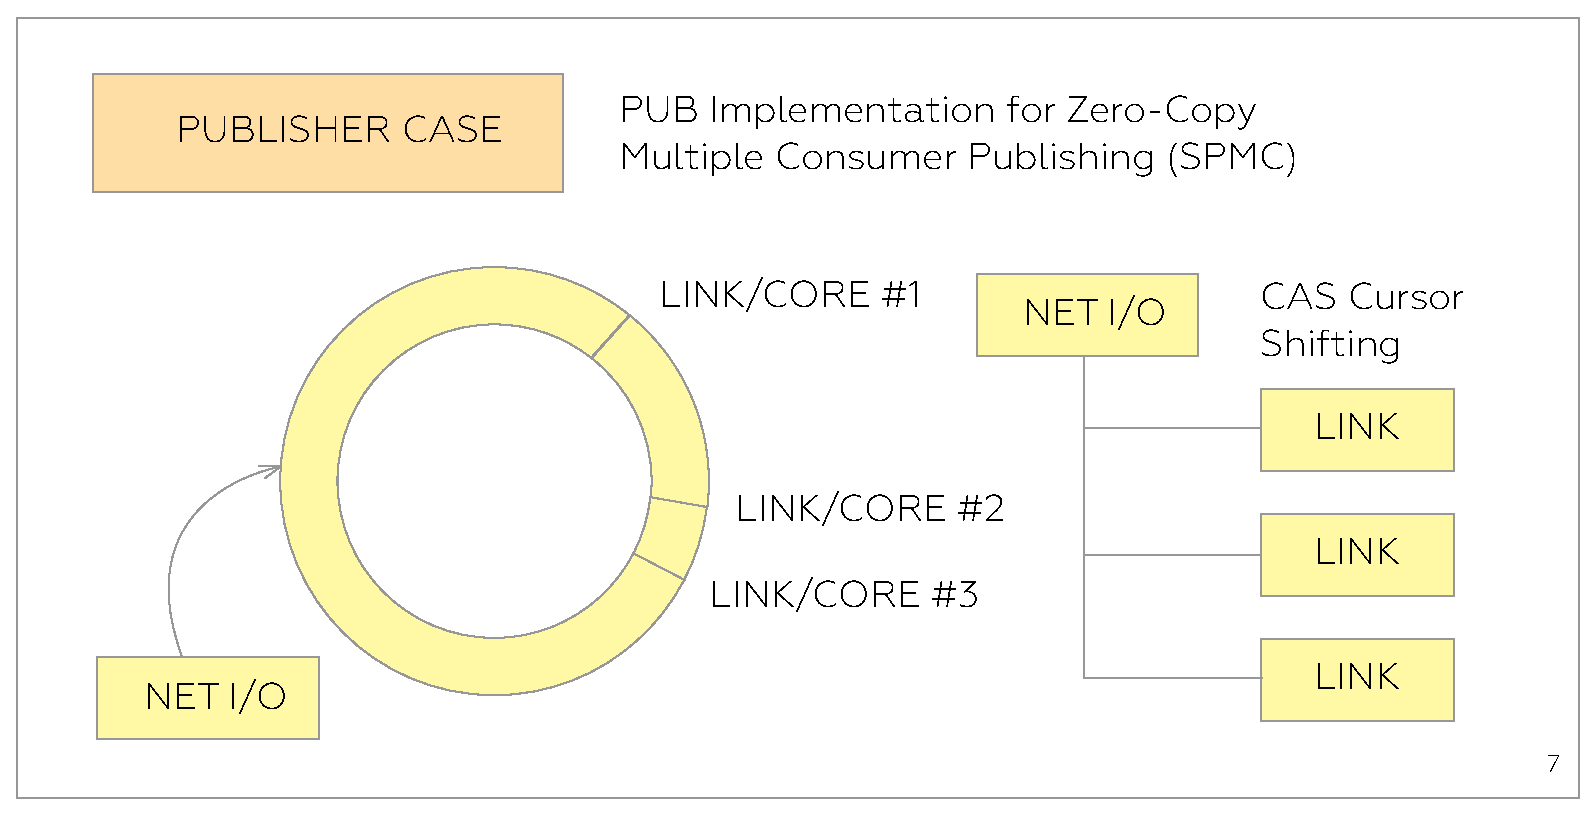
\includegraphics[scale=0.25]{pub.eps}}
  \caption{Кільцева статична черга з CAS-курсором для публікації}
\end{figure}
Для забезпечення імутабельності (нерухомості даних) та відсутності
копіювання в подальшій роботі, дані залишаються в черзі, а рухаються та передаються
лише курсори на типизовані послідовності даних.
\begin{figure}[h]
  \centerline{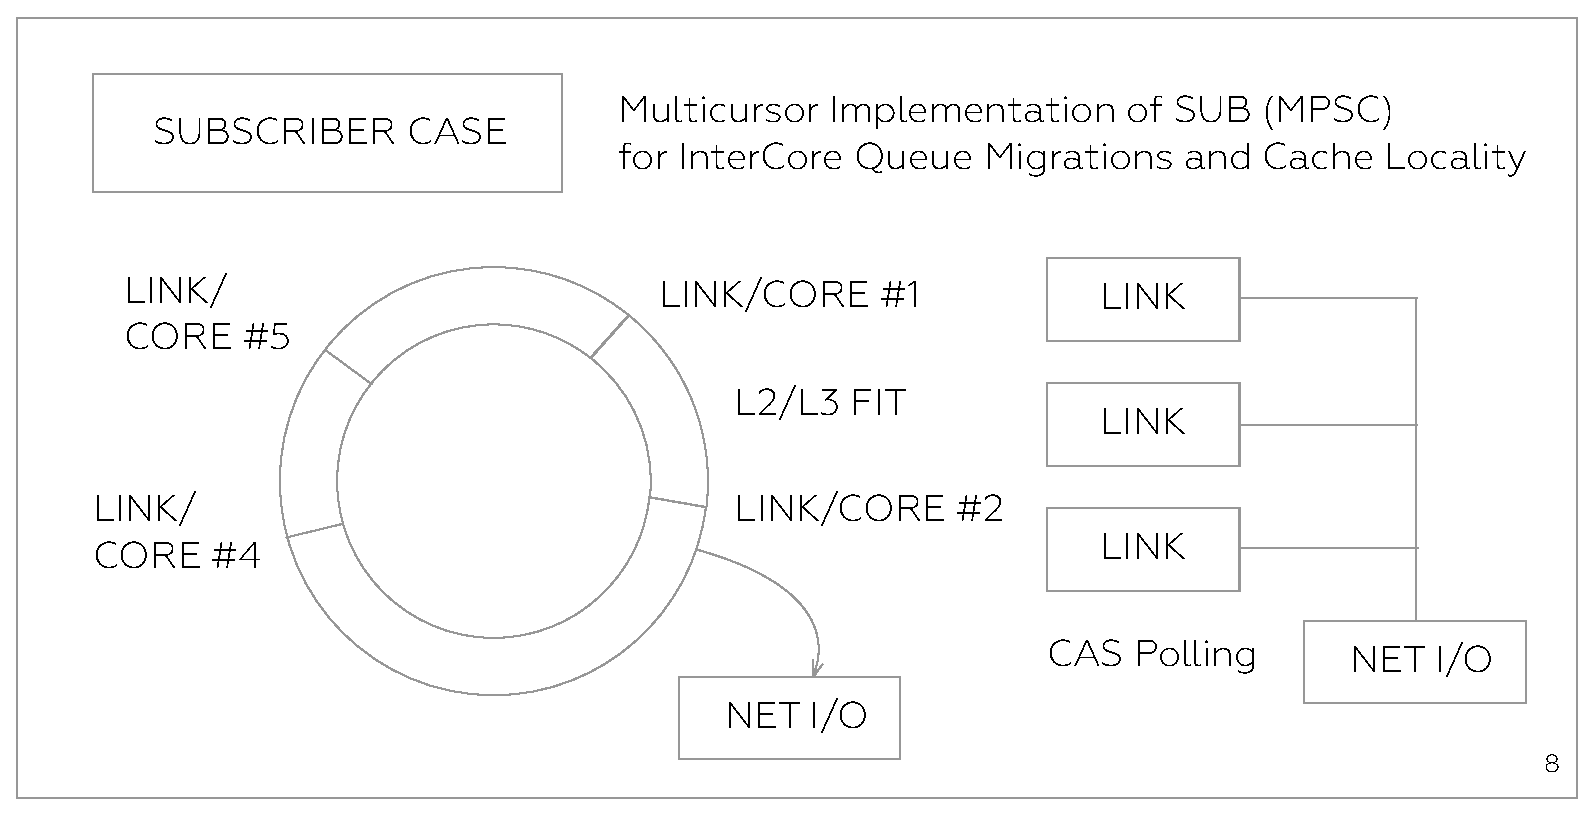
\includegraphics[scale=0.25]{sub.eps}}
  \caption{Кільцева статична черга з CAS-курсором для згортки}
\end{figure}

\subsubsection{Реактори}
Кожен процесор має три типи реакторів які можуть бути на ньому запущені:
i) Task-реактор; ii) Timer-реактор; iii) IO-цикли. Для Task-реактора
існують черги пріорітетів, а для Timer-реактора --- дерева інтервалів.
\begin{figure}[h]
  \centerline{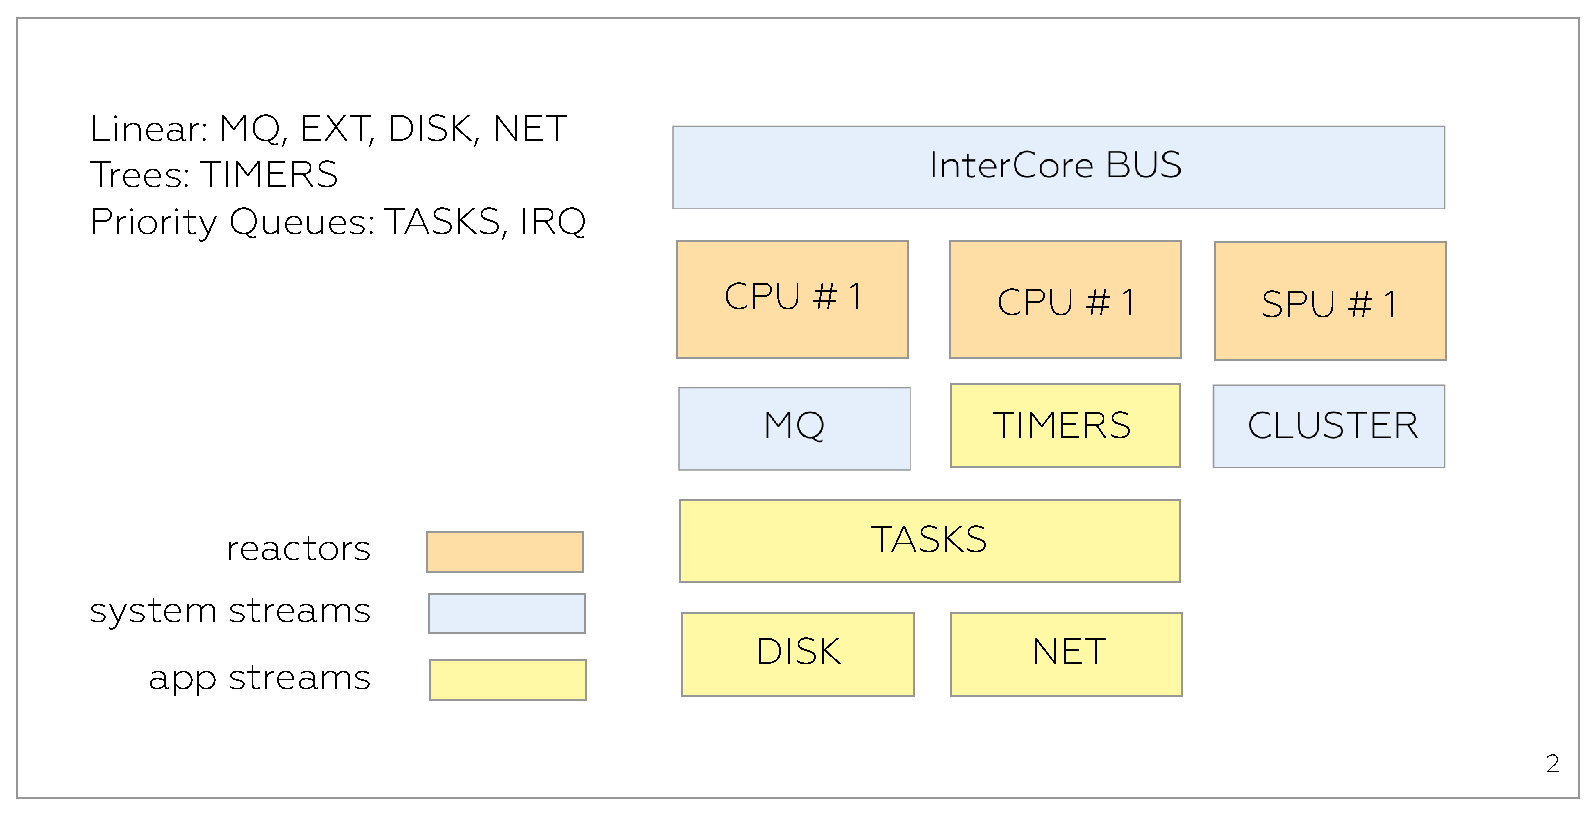
\includegraphics[scale=0.25]{sys.eps}}
  \caption{Система процесорних ядер та реакторів}
\end{figure}
Загальний спосіб комунікації для задач виглядає як публікація
в чергу (рух курсора запису) та підписка на черги і
згортання (руху курсора читання). Кожна черга має як
курсори для публікації так і курсори для читання. Можливо також
використання міжреакторної шини InterCore та посилання
службового повідомлення по цій шині на інший реактор. Так,
наприклад, працюють таймери та старти процесів, які передають
сигнал в реактор для перепланування. Можна створювати нові повідомлення
шини InterCore і систему фільтрів для згортання черги
реактора для більш гнучкої обробки сигналів реального часу.

\subsubsection*{Task-реактор}
Task-реактор або реактор задач виконує Rust задачі або
програми інтерпретатора, які можуть бути двох видів:
кінечні (які повертають результат виконання),
або бескінечні (процеси).
%\begin{figure}[h]
%  \centerline{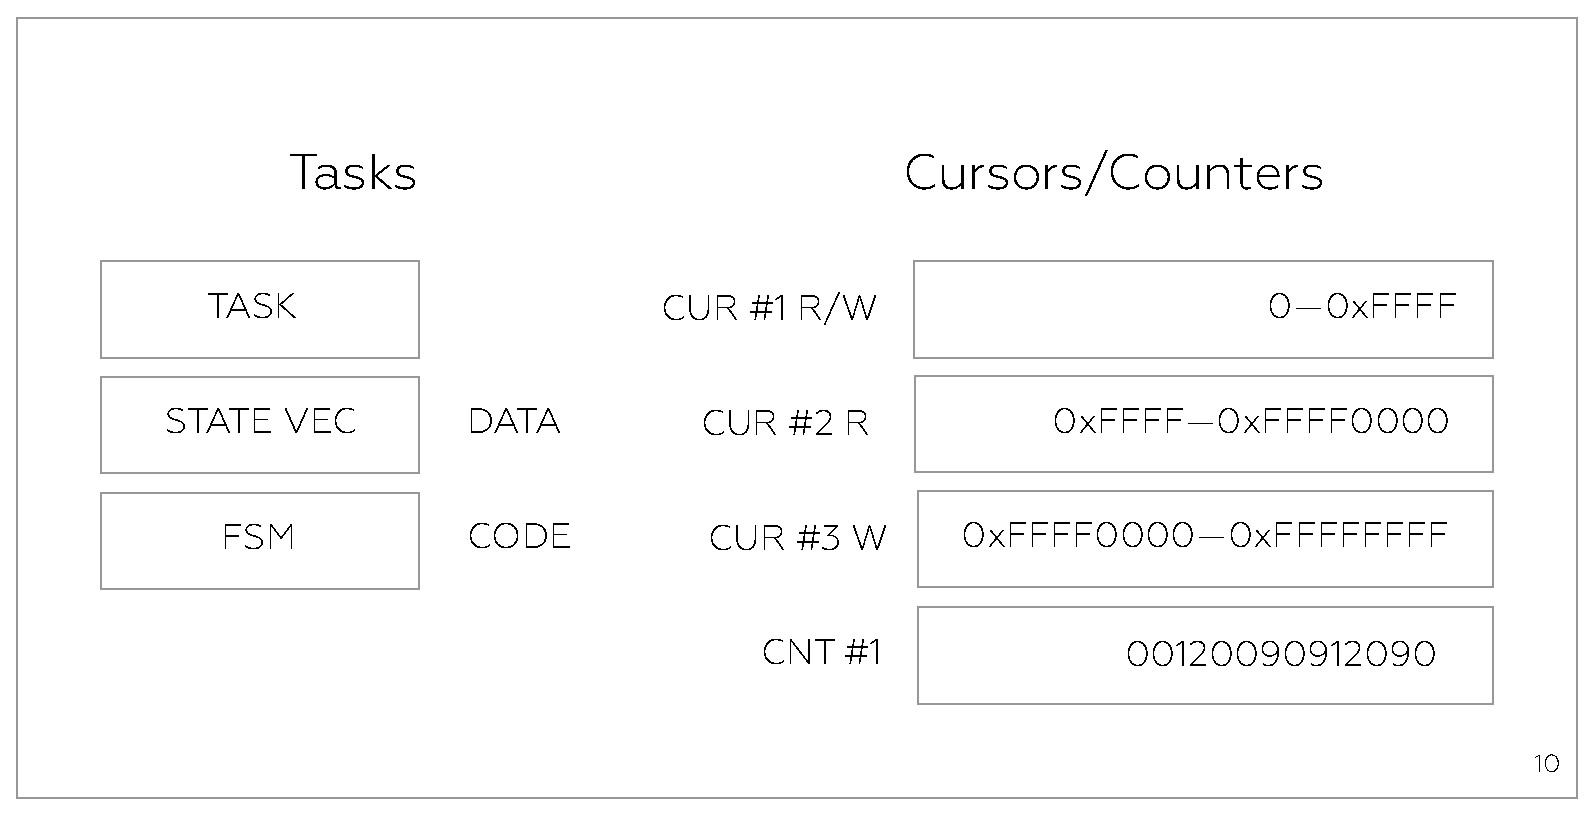
\includegraphics[scale=0.25]{task.eps}}
%  \caption{Task-реактор або система інтерпретаторів}
%\end{figure}

Приклад бескінечної задачі --- 0-процес,
який запускається при старті системи. Цей процес завжди доступний
по WebSocket каналу та з консолі терміналу.

\subsubsection*{IO-реактор}
Мережевий сервер або IO-реактор може обслуговувати багато
мережевих з'єднань та підтримує Windows, Linux, Mac смаки.
%\begin{figure}[h]
%  \centerline{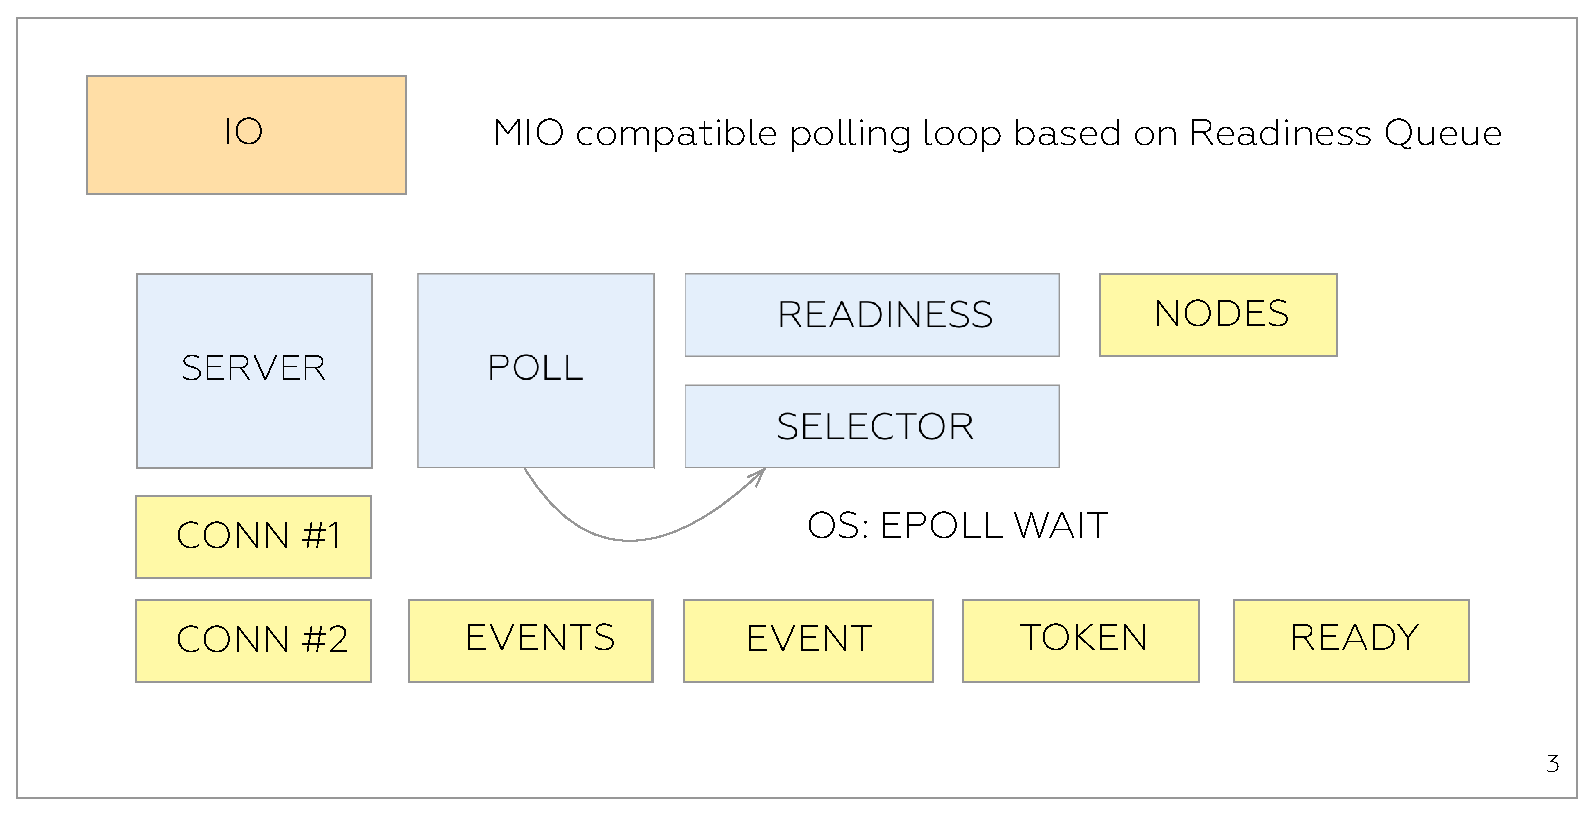
\includegraphics[scale=0.25]{net.eps}}
%  \caption{IO-реактор або процес опитування мережевих сервісів}
%\end{figure}

\subsubsection*{Timer-реактор}
Різні типи сутностей планування (такі як Task, IO, Timer)
мають різні дисципліни селекторів повідомлень для черг
(послідовно, через само-балансуючі дерева, BTree дерева тощо).
%\begin{figure}[h]
%  \centerline{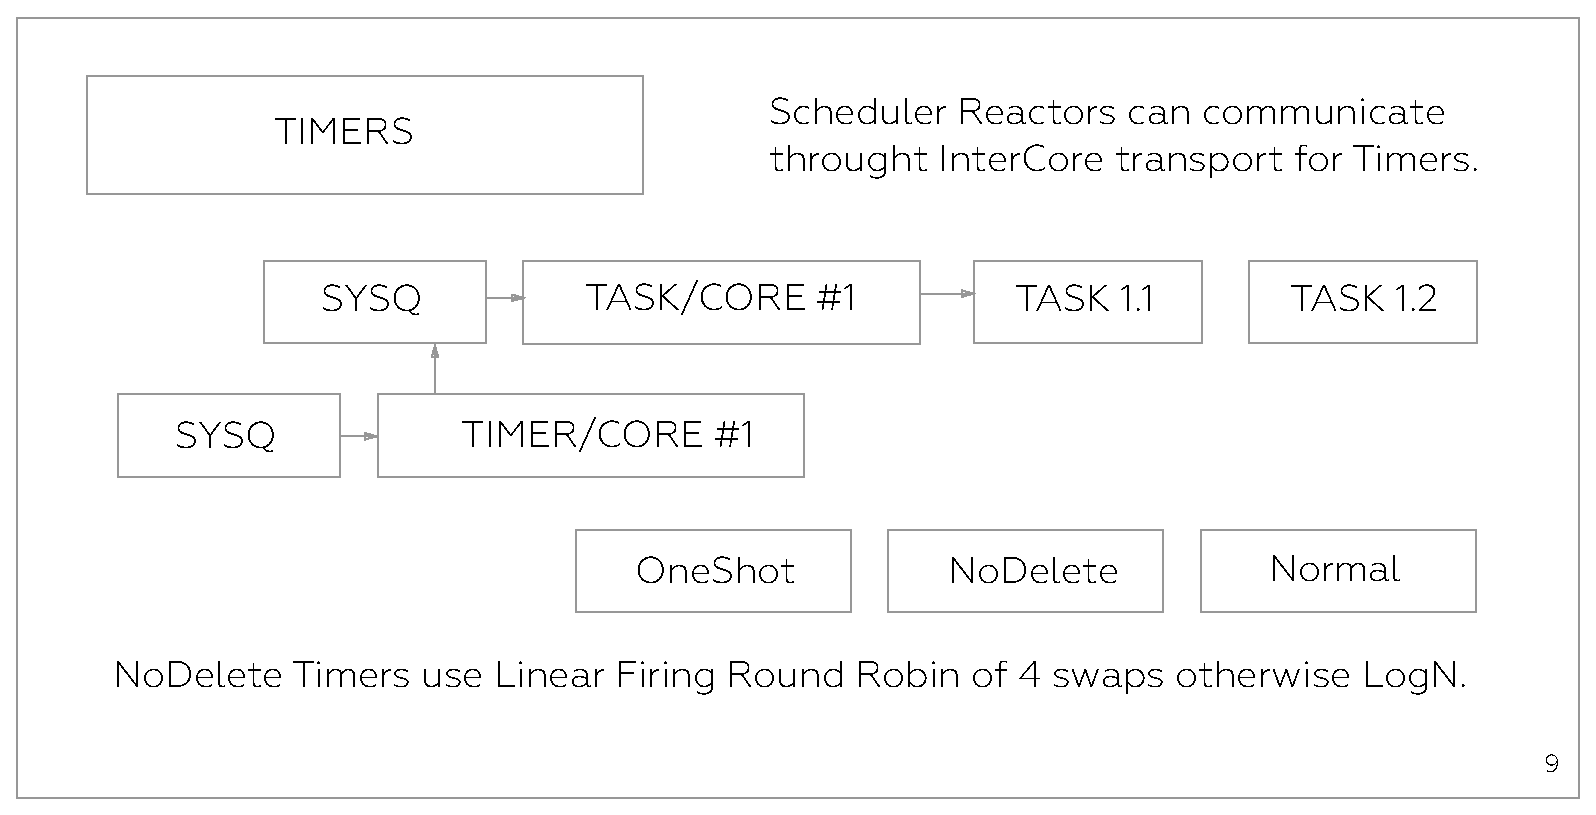
\includegraphics[scale=0.25]{timer.eps}}
%  \caption{Timer-реактор або драйвер процесорного таймеру}
%\end{figure}

\subsubsection{Міжреакторний транспорт InterCore}
Шина InterCore конструюється певним числом SPMC черг, виділених для певного ядра.
Шина сама має топологію зірки між ядрами, та черга MPSC організована
як функція над множиною паблішерів. Кожне ядро має рівно одного паблішера.
Функція обробки шини протоколу InterCore називається poll\_bus та є членом планувальника.
Ви можете думати про InterCore як телепорт між процесорами, так як pull\_bus
викликається після кожної операції Yield в планувальник, і, таким чином,
якщо певному ядру опублікували в його чергу повідомлення, то після наступного Yield
на цьому ядрі буде виконана функція обробки цього повідомлення.

\subsubsection*{\lstinline{pub [ capacity ]}}
Створює новий CAS курсор для паблішінга, тобто для запису.
Повертає глобальних машинний ідентифікатор, має єдиний параметр, розмір черги.
Приклад: p: pub[16].

\subsubsection*{\lstinline{sub [ publisher ]}}
Створює новий CAS курсор для читання певної черги, певного врайтера.
Повертає глобальний машинний ідентифікатор для читання.
Приклад: s: sub[p].

\subsubsection*{\lstinline{spawn [ core ; program ; cursors ]}}
Створює нову програму задачу CPS-інтепреторатора для певного ядра.
Задача може бути або програмою на мові Rust або будь якою програмою через FFI.
Також при створенні задачі задається список курсорів,
які ексклюзивно належатимуть до цієї задачі.
Параметри функції: ядро, текст програми або назва FFI функції,спсисок курсорів.
Приклад: spawn[0;"etc/proc0";(0;1)].

\subsubsection*{\lstinline{snd [ writer ; data ]}}
Посилає певні дані в певний курсор для запису. Повертає Nil якшо всьо ОК.
Приклад: snd[p;42].

\subsubsection*{\lstinline{rcv [ reader ]}}
Повертає прочитані дані з певного курсору.
Якшо даних немає, то передає управління в планувальних за допомогою Yield.
Приклад: rcv[s].

\subsection{Структури ядра}
Ядро є ситемою акторів з двома основними типами акторів:
чергами, які представляють кільцеві буфери та відрізки памяті;
та задачами, які резпрезентують байт-код програм та іх інтерпретацію на процесорі.
Черги бувають двох видів: для публікації, які місять курсори для запису;
та для читання, які містять курсори для читання. Задачі можна імплементувати
як Rust програми, або як $O_{CPS}$ програми.

\subsubsection{Черга для публікації}
\begin{lstlisting}
pub struct Publisher<T> {
    ring: Arc<RingBuffer<T>>,
    next: Cell<Sequence>,
    cursors: UncheckedUnsafeArc<Vec<Cursor>>,
}
\end{lstlisting}

\subsubsection{Черга для читання}
\begin{lstlisting}
pub struct Subscriber<T> {
    ring: Arc<RingBuffer<T>>,
    token: usize,
    next: Cell<Sequence>,
    cursors: UncheckedUnsafeArc<Vec<Cursor>>,
}
\end{lstlisting}

Існує дві спецільні задачі: InterCore задача, написана на Rust,
та запускається на всіх ядрах при запуску системи, а також CPS-інтерпретор
головного термінала системи, цей інтерпретор запускається на BSP ядрі,
поближче до Console та WebSocket IO селекторів.
В процесі життя різні CPS та Rust задачі можуть бути запущені в такій системі,
поєднуючи гнучкість програм інтерпретатора, та низькорівненивих програм написаних на мові Rust.

Окрім черг та задач, в системі присутні також таймери та інші IO задачі,
такі як сервери мережі або сервери доступу до файлів. Також існують
структури які репрезентують ядра та містять палнувальники.
Уся віртуальна машина є сукупністю таких структур-ядер.

\subsubsection{Канал}
Канал складається з одного курсору для запису та багатьох курсорів для читання.
Канал предствляє собою компонент зірки шини InterCore.
\begin{lstlisting}
pub struct Channel {
    publisher: Publisher<Message>,
    subscribers: Vec<Subscriber<Message>>,
}
\end{lstlisting}

\subsubsection{Черги ядра}
Память репрезентує усі наявні черги для публікації та читання на ядрі.
Ця інформація передається клонованою кожній задачі планувальника на цьому ядрі.
\begin{lstlisting}
pub struct Memory<'a> {
    publishers: Vec<Publisher<Value<'a>>,
    subscribers: Vec<Subscriber<Value<'a>>>,
}
\end{lstlisting}

\subsubsection{Планувальник}
Планувальник репрезентує ядро процесара,
які розрізняються як BSP-ядра (або 0-ядра, bootstrap)
та AP ядра (інші ядра > 0, application). BSP ядро
тримає на собі Console та WebSocket IO селектори.
Це означає, що BSP ядро дає свій час на обробку зовнішньої інформації,
у той час як AP процесори не обтяжені
таким навантаженням (io черга в таких планувальниках пуста).
Існує InterCore повідомлення яке додає або видаляє довільні IO селектори
в планувальних для довільних конфігурацій.

\begin{lstlisting}
pub struct Scheduler<'a> {
    pub tasks: Vec<T3<Job<'a>>>,
    pub bus: Channel,
    pub queues: Memory<'a>,
    pub io: IO,
}
\end{lstlisting}

\subsection{Протокол InterCore}
Протокол шини InterCore.

\begin{lstlisting}
pub enum Message {
    Pub(Pub),
    Sub(Sub),
    Print(String),
    Spawn(Spawn),
    AckSub(AckSub),
    AckPub(AckPub),
    AckSpawn(AckSpawn),
    Exec(usize, String),
    Select(String, u16),
    QoS(u8, u8, u8),
    Halt,
    Nop,
}
\end{lstlisting}

\section{Висновки}
Як апогей, система HTS є фінальною категорією,
куди сходяться всі стрілки категорії мов. Кожна мова та її категорія
мають певний набір стрілок ендоморфізмів, які обчислюють, верифікують,
нормалізують, оптимізують програми своїх мов.
Стрілки виду $e_i: O_{n+1} \rightarrow O_n$ є екстракторами, які понижають систему типів,
при чому $O_{CPS} = O_0$.

Базова бібліотека мови Ерланг в яку проводиться основний
естракт йде з дистрибутивом Erlang/OTP. Базова бібліотека
$O_{PTS}$ наведена в репозиторії Github\footnote{\url{https://github.com/groupoid/om}}.
Гомотопічна базова бібліотека відповідає термінальній мові $O_{CCHM}$, та теж відкрита
на Github\footnote{\url{https://github.com/groupoid/infinity}}.
Останні два розділи присвячені математичному моделюванню математики на цій мові.

\subsection{Базова бібліотека}
Перша частина гомотопічної базової бібліотеки --- це основи гомотопічної теорії типів,
з основними визначеннями та теоремами.

\subsection{Математичні компоненти}
Друга частина гомотопічної базової бібліотеки --- це формалізація математики, як
приклад використання розробленої концепцтуальної моделі системи доведення теорем.

